\documentclass[pdf]{beamer}
\usepackage{graphicx}
\mode<presentation>{}
\title{LibEuFin}
\subtitle{Libre European Finance}
\author{Marcello Stanisci}

\begin{document}

% Notes:
% What's missing:
% - make clear why this is *civic tech*
%   (e.g.: moving away from 3rd party surveillance,
%    moving away from cloud, taking control of your own (bank transaction) data)
% - make more clear how other civic tech projects can benefit

% Title frame
\begin{frame}
  \titlepage
\end{frame}

\begin{frame}
  \begin{center}
  People and businesses need programmatic access to bank accounts, and
  the EU recognized this by passing the 2nd Payment Service Directive.

  But it's extremely complicated!
  \end{center}
\end{frame}

\begin{frame}{Too many protocols..}
  \begin{itemize}
    \item EBICS: hundreds of pages, just for {\it enclosing} payloads
    \item ISO20022: hundreds of pages for payloads
    \item FinTS / HBCI: hundreds of pages
    \item NextGenPSD2 by Berlin Group 
    \item Startup banks: N26 / Revoult
    \item 100\% proprietary: PayPal
    \item ..
  \end{itemize}
\end{frame}

\begin{frame}{LibEuFin}
  \begin{center}
  LibEuFin is an Open Source service and API that allows developers
  communities and SMEs to programmatically access their bank accounts.

  It abstracts over complex legacy APIs and provides a bank sandbox
  to make testing cheap and easy.
  \end{center}
\end{frame}

\begin{frame}{Improvements}
  \begin{itemize}
  \item {\it Unifies} several banking protocols into an abstraction layer.
  \item Enables development of FinTech apps {\it without clouds or third parties}
  \item {\it Frees} application developers from implementing {\it difficult cryptography}
  \end{itemize}
\end{frame}

\begin{frame}{Architecture}
  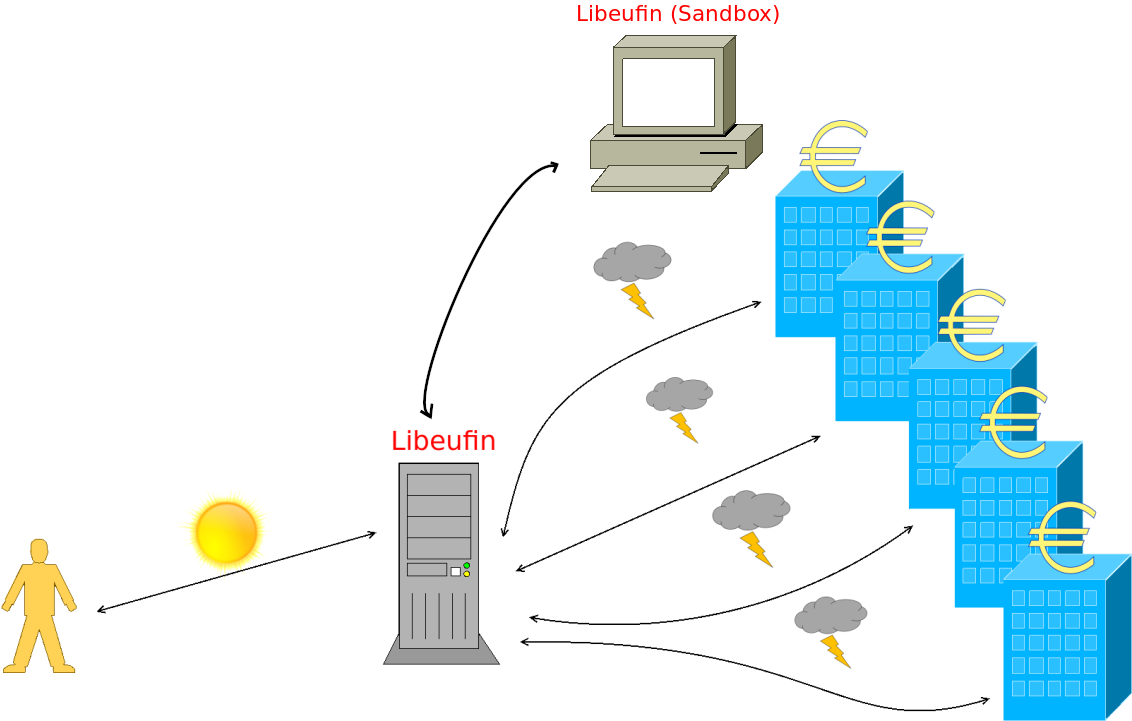
\includegraphics[height=0.63\textheight]{libeufin.png}
\end{frame}

\begin{frame}{Current status}
  \begin{itemize}
    \item One major protocol (EBICS) implemented
    \item Current code works with real GLS bank account!
    \item Should work with all banks of the German Credit Union (DK)
    \item Ongoing integration with Taler (former PF project).
  \end{itemize}
\end{frame}

\begin{frame}{Challenges}
  \begin{itemize}
    \item Slow communication with banks.
    \item Difficult protocols and documentations.
    \item Subscriber initiation process.
    \item No testing environment available.
  \end{itemize}
\end{frame}

\begin{frame}{Successes}
  \begin{itemize}
    \item Milestones estimation was (almost!) accurate.
    \item Our approach to testing (develop sandbox first) was successful: Real bank access
          worked on first try, after 4 months of development.
  \end{itemize}
\end{frame}

\begin{frame}{What did we learn?}
  \begin{center}
  We believe that \textbf{simplicity} is the key for any system to
  properly function, and that is LibEuFin primary goal.
  \end{center}
\end{frame}

\end{document}
